% LaTeX support: latex@mdpi.com 
% In case you need support, please attach all files that are necessary for compiling as well as the log file, and specify the details of your LaTeX setup (which operating system and LaTeX version / tools you are using).

%=================================================================
\documentclass[energies,article,submit,moreauthors,pdftex]{Definitions/mdpi} 
% \usepackage{graphics}
\usepackage{amsthm, amssymb, amsfonts}
\usepackage{array,longtable}
\usepackage{overpic}
\graphicspath{{./Images/}}
% If you would like to post an early version of this manuscript as a preprint, you may use preprint as the journal and change 'submit' to 'accept'. The document class line would be, e.g., \documentclass[preprints,article,accept,moreauthors,pdftex]{mdpi}. This is especially recommended for submission to arXiv, where line numbers should be removed before posting. For preprints.org, the editorial staff will make this change immediately prior to posting.

%--------------------
% Class Options:
%--------------------
%----------
% journal
%----------
% Choose between the following MDPI journals:
% acoustics, actuators, addictions, admsci, aerospace, agriculture, agriengineering, agronomy, algorithms, animals, antibiotics, antibodies, antioxidants, applsci, arts, asc, asi, atmosphere, atoms, axioms, batteries, bdcc, behavsci, beverages, bioengineering, biology, biomedicines, biomimetics, biomolecules, biosensors, brainsci, buildings, cancers, carbon, catalysts, cells, ceramics, challenges, chemengineering, chemistry, chemosensors, children, cleantechnol, climate, clockssleep, cmd, coatings, colloids, computation, computers, condensedmatter, cosmetics, cryptography, crystals, dairy, data, dentistry, designs, diagnostics, diseases, diversity, drones, econometrics, economies, education, ejihpe, electrochem, electronics, energies, entropy, environments, epigenomes, est, fermentation, fibers, fire, fishes, fluids, foods, forecasting, forests, fractalfract, futureinternet, futurephys, galaxies, games, gastrointestdisord, gels, genealogy, genes, geohazards, geosciences, geriatrics, hazardousmatters, healthcare, heritage, highthroughput, horticulturae, humanities, hydrology, ijerph, ijfs, ijgi, ijms, ijns, ijtpp, informatics, information, infrastructures, inorganics, insects, instruments, inventions, iot, j, jcdd, jcm, jcp, jcs, jdb, jfb, jfmk, jimaging, jintelligence, jlpea, jmmp, jmse, jnt, jof, joitmc, jpm, jrfm, jsan, land, languages, laws, life, literature, logistics, lubricants, machines, magnetochemistry, make, marinedrugs, materials, mathematics, mca, medicina, medicines, medsci, membranes, metabolites, metals, microarrays, micromachines, microorganisms, minerals, modelling, molbank, molecules, mps, mti, nanomaterials, ncrna, neuroglia, nitrogen, notspecified, nutrients, ohbm, optics, particles, pathogens, pharmaceuticals, pharmaceutics, pharmacy, philosophies, photonics, physics, plants, plasma, polymers, polysaccharides, preprints, proceedings, processes, proteomes, psych, publications, quantumrep, quaternary, qubs, reactions, recycling, religions, remotesensing, reports, resources, risks, robotics, safety, sci, scipharm, sensors, separations, sexes, signals, sinusitis, smartcities, sna, societies, socsci, soilsystems, sports, standards, stats, surfaces, surgeries, sustainability, symmetry, systems, technologies, test, toxics, toxins, tropicalmed, universe, urbansci, vaccines, vehicles, vetsci, vibration, viruses, vision, water, wem, wevj

%---------
% article
%---------
% The default type of manuscript is "article", but can be replaced by: 
% abstract, addendum, article, benchmark, book, bookreview, briefreport, casereport, changes, comment, commentary, communication, conceptpaper, conferenceproceedings, correction, conferencereport, expressionofconcern, extendedabstract, meetingreport, creative, datadescriptor, discussion, editorial, essay, erratum, hypothesis, interestingimages, letter, meetingreport, newbookreceived, obituary, opinion, projectreport, reply, retraction, review, perspective, protocol, shortnote, supfile, technicalnote, viewpoint
% supfile = supplementary materials

%----------
% submit
%----------
% The class option "submit" will be changed to "accept" by the Editorial Office when the paper is accepted. This will only make changes to the frontpage (e.g., the logo of the journal will get visible), the headings, and the copyright information. Also, line numbering will be removed. Journal info and pagination for accepted papers will also be assigned by the Editorial Office.

%------------------
% moreauthors
%------------------
% If there is only one author the class option oneauthor should be used. Otherwise use the class option moreauthors.

%---------
% pdftex
%---------
% The option pdftex is for use with pdfLaTeX. If eps figures are used, remove the option pdftex and use LaTeX and dvi2pdf.

%=================================================================
\firstpage{1} 
\makeatletter 
\setcounter{page}{\@firstpage} 
\makeatother
\pubvolume{xx}
\issuenum{1}
\articlenumber{5}
\pubyear{2019}
\copyrightyear{2019}
%\externaleditor{Academic Editor: name}
\history{Received: date; Accepted: date; Published: date}
%\updates{yes} % If there is an update available, un-comment this line

%% MDPI internal command: uncomment if new journal that already uses continuous page numbers 
%\continuouspages{yes}

%------------------------------------------------------------------
% The following line should be uncommented if the LaTeX file is uploaded to arXiv.org
%\pdfoutput=1

%=================================================================
% Add packages and commands here. The following packages are loaded in our class file: fontenc, calc, indentfirst, fancyhdr, graphicx, lastpage, ifthen, lineno, float, amsmath, setspace, enumitem, mathpazo, booktabs, titlesec, etoolbox, amsthm, hyphenat, natbib, hyperref, footmisc, geometry, caption, url, mdframed, tabto, soul, multirow, microtype, tikz

% \PassOptionsToPackage[OT1]{fontenc} % options for packages loaded elsewhere
%=================================================================
%% Please use the following mathematics environments: Theorem, Lemma, Corollary, Proposition, Characterization, Property, Problem, Example, ExamplesandDefinitions, Hypothesis, Remark, Definition, Notation, Assumption
%% For proofs, please use the proof environment (the amsthm package is loaded by the MDPI class).

%=================================================================
% Full title of the paper (Capitalized)
\Title{Revealing trends in geophysics using metadata analysis}

% Author Orchid ID: enter ID or remove command
\newcommand{\orcidauthorA}{0000-0002-7928-5736} % Add \orcidA{} behind the author's name
\newcommand{\orcidauthorB}{0000-0002-9743-7107} % Add \orcidB{} behind the author's name
\newcommand{\orcidauthorC}{0000-0002-9389-7579} % Add \orcidB{} behind the author's name

% Authors, for the paper (add full first names)
\Author{Timofey Eltsov $^{1,\dagger}$\orcidA{}, Maxim Yutkin $^{2}$\orcidB{}, Tadeusz W. Patzek $^{3}$\orcidC{}} % and Firstname Lastname $^{2,}$*}

% Authors, for metadata in PDF
\AuthorNames{Timofey Eltsov and Tadeusz W. Patzek}

% Affiliations / Addresses (Add [1] after \address if there is only one affiliation.)
\address{$^{1}$ \quad Ali I. Al-Naimi Petroleum Engineering Research Center, King Abdullah University of Science and Technology; timofey.eltsov@kaust.edu.sa\\
$^{2}$ \quad Ali I. Al-Naimi Petroleum Engineering Research Center, King Abdullah University of Science and Technology; maxim.yutkin@kaust.edu.sa\\
$^{3}$ \quad Ali I. Al-Naimi Petroleum Engineering Research Center, King Abdullah University of Science and Technology; tadeusz.patzek@kaust.edu.sa}

% Contact information of the corresponding author
\corres{Correspondence: timofey.eltsov@kaust.edu.sa; Tel.: +966128087182}

% Current address and/or shared authorship
\firstnote{Current address: 4700 KAUST, Thuwal, 23955-6900, Saudi Arabia}
% The commands \thirdnote{} till \eighthnote{} are available for further notes

%\simplesumm{} % Simple summary

%\conference{} % An extended version of a conference paper

% Abstract (Do not insert blank lines, i.e. \\) 
\abstract{Computing power is limited in its capacity to process the ever increasing available data. The information space is so clogged that it is often impossible to find the necessary data among millions of terabytes. Amidst all the  the abundance of information, we propose to turn to the analysis of metadata of publications in the geophysical field of knowledge. An analysis of the publication activity of oil producing and oilfield service companies will shed light on the state of the geophysical market. Here, we describe the  metadata analysis of the last 38 Annual Conferences organized by the Society of Exploration Geophysicists, one of the biggest geophysical gatherings. The number of publications from industrial companies in the energy sector has a direct link with the financial situation. Publications from the academia of various countries tell us about state funding of research in each country and indirectly reflect the geopolitical situation in the world. The changing number of publications over time shows us the dynamics of the transformation of the geophysical market and allows us to understand what is happening and make forecasts. In 2018, Schlumberger and Saudi Aramco had the highest number of publications among service and production companies. In 2019, BGP and PetroChina took the lead. Throughout history, the USA academia have had the highest number of publications but in 2019 the Chinese academia came close to taking the lead.}


% Keywords
\keyword{geophysics; web data analysis; data mining; data analysis; metadata analysis}

% The fields PACS, MSC, and JEL may be left empty or commented out if not applicable
%\PACS{J0101}
%\MSC{}
%\JEL{}

%%%%%%%%%%%%%%%%%%%%%%%%%%%%%%%%%%%%%%%%%%
% Only for the journal Diversity
%\LSID{\url{http://}}

%%%%%%%%%%%%%%%%%%%%%%%%%%%%%%%%%%%%%%%%%%
% Only for the journal Applied Sciences:
%\featuredapplication{Authors are encouraged to provide a concise description of the specific application or a potential application of the work. This section is not mandatory.}
%%%%%%%%%%%%%%%%%%%%%%%%%%%%%%%%%%%%%%%%%%

%%%%%%%%%%%%%%%%%%%%%%%%%%%%%%%%%%%%%%%%%%
% Only for the journal Data:
%\dataset{DOI number or link to the deposited data set in cases where the data set is published or set to be published separately. If the data set is submitted and will be published as a supplement to this paper in the journal Data, this field will be filled by the editors of the journal. In this case, please make sure to submit the data set as a supplement when entering your manuscript into our manuscript editorial system.}

%\datasetlicense{license under which the data set is made available (CC0, CC-BY, CC-BY-SA, CC-BY-NC, etc.)}

%%%%%%%%%%%%%%%%%%%%%%%%%%%%%%%%%%%%%%%%%%
% Only for the journal Toxins
%\keycontribution{The breakthroughs or highlights of the manuscript. Authors can write one or two sentences to describe the most important part of the paper.}

%\setcounter{secnumdepth}{4}
%%%%%%%%%%%%%%%%%%%%%%%%%%%%%%%%%%%%%%%%%%
\begin{document}
%%%%%%%%%%%%%%%%%%%%%%%%%%%%%%%%%%%%%%%%%%

%%%%%%%%%%%%%%%%%%%%%%%%%%%%%%%%%%%%%%%%%%
% \setcounter{section}{-1} %% Remove this when starting to work on the template.
%\section{How to Use this Template}
%The template details the sections that can be used in a manuscript. Note that the order and names of article sections may differ from the requirements of the journal (e.g., the positioning of the Materials and Methods section). Please check the instructions for authors page of the journal to verify the correct order and names. For any questions, please contact the editorial office of the journal or support@mdpi.com. For LaTeX related questions please contact latex@mdpi.com.
%%The order of the section titles is: Introduction, Materials and Methods, Results, Discussion, Conclusions for these journals: aerospace,algorithms,antibodies,antioxidants,atmosphere,axioms,biomedicines,carbon,crystals,designs,diagnostics,environments,fermentation,fluids,forests,fractalfract,informatics,information,inventions,jfmk,jrfm,lubricants,neonatalscreening,neuroglia,particles,pharmaceutics,polymers,processes,technologies,viruses,vision

\section{Introduction}

The amount of data is constantly increasing over the years. In 2018 the total estimated size of the Datasphere was 33 zettabytes (ZB) with a pridiction of 175 ZB in 2025 \citep{Reinsel2018}. Utilization of one GB of information was estimated to be 5.12 kWh \citep{Costenaro2012}. It was about \$0.51 back in 2012. It should be noted that in 2012 Information and Communication Technology (ICT) related products and services accounted for 4.6\% of worldwide electricity consumption \citep{Heddeghem2014} and it keeps growing. The global electricity demand on data centers in 2018 was estimated to be 198 TWh, which is almost 1\% of the global final demand for electricity \citep{Dulac2019}. Wherein Swedish KTH\footnote{KTH Royal Institute of Technology in Stockholm} report indicate that  about  10\% of the world’s total electricity consumption is being used by the internet \citep{KTH2019}. Estimated increase in datasphere size suggests an inevitable increase in energy consumption over time. In this case, an almost linear increase in energy consumption can be assumed. BP, in  its review on world energy, reports that in 2019, 84\% of the total energy was produced by burning coal, natural gas, and oil \citep{BP2019}. The 16\% was produced by nuclear, hydro, and renewables. Therefore, we can say that a five-fold increase in the datasphere will require a five-fold increase in the burning of valuable hydrocarbons by 2025. Researchers are inclined to argue that the amount of data is only growing, and we are generating ``informational debt.'' Only a small part of the information is being processed, leaving the bulk for storage. If in doubt, remember the last time you sorted photos from your phone and deleted unnecessary ones. The authors ask you to think, is it time to process the accumulated information debt and draw important conclusions?

Data processing itself is important, but also new approaches to processing are crucial. Here we analyze the geophysical market based on the proceedings of the Society of Exploration Geophysicists (SEG) Annual Conferences. To understand the changes in the energy sector, the geophysical market is very important, because it is geophysicists who find and explore the mineral deposits on which our civilization is based. Changes in the geophysics sector with a time delay triggers a response in the energy sector. The SEG Annual Conference and Exhibition is one of the most significant gatherings of geophysicists in the world. A presentation at this conference raises the prestige of companies and shows the scientific viability of academic institutions. These conferences have been held annually for many decades and we have access to online conference materials over the past 38 years \citep{SEG}. Researchers and engineers report on their cutting-edge developments, and so we get an annual account of the most relevant technologies. We see that the number of publications from oil and oilfield service companies reflects their economic situation on the market, and the number of publications from academia in various countries speaks of state funding for scientific work. The authors have not seen such an approach to the processing of published materials, and we suggest the possibility of using our approach in other areas. 


%%%%%%%%%%%%%%%%%%%%%%%%%%%%%%%%%%%%%%%%%%%
\section{Materials and Methods}

We used the OnePetro online library \citep{SPE2019} to get metadata of the reviewed papers. The OnePetro website offers ample opportunities for analyzing metadata. Along with OnePetro, CrossRef service can be used for metadata analysis. Different spelling versions and typos affected the study of affiliation. Besides, many organizations have since ceased to exist (acquired, bankrupt, split, \textit{etc.}), which also complicated the analysis. We use open-source Python libraries to get and process metadata: Requests-HTML, sqlite3, and NumPy. For printing the graphs, we use Matplotlib, Plotly, PIL (Python Imaging Library), and others.


\begin{figure}[ht!]
\centering
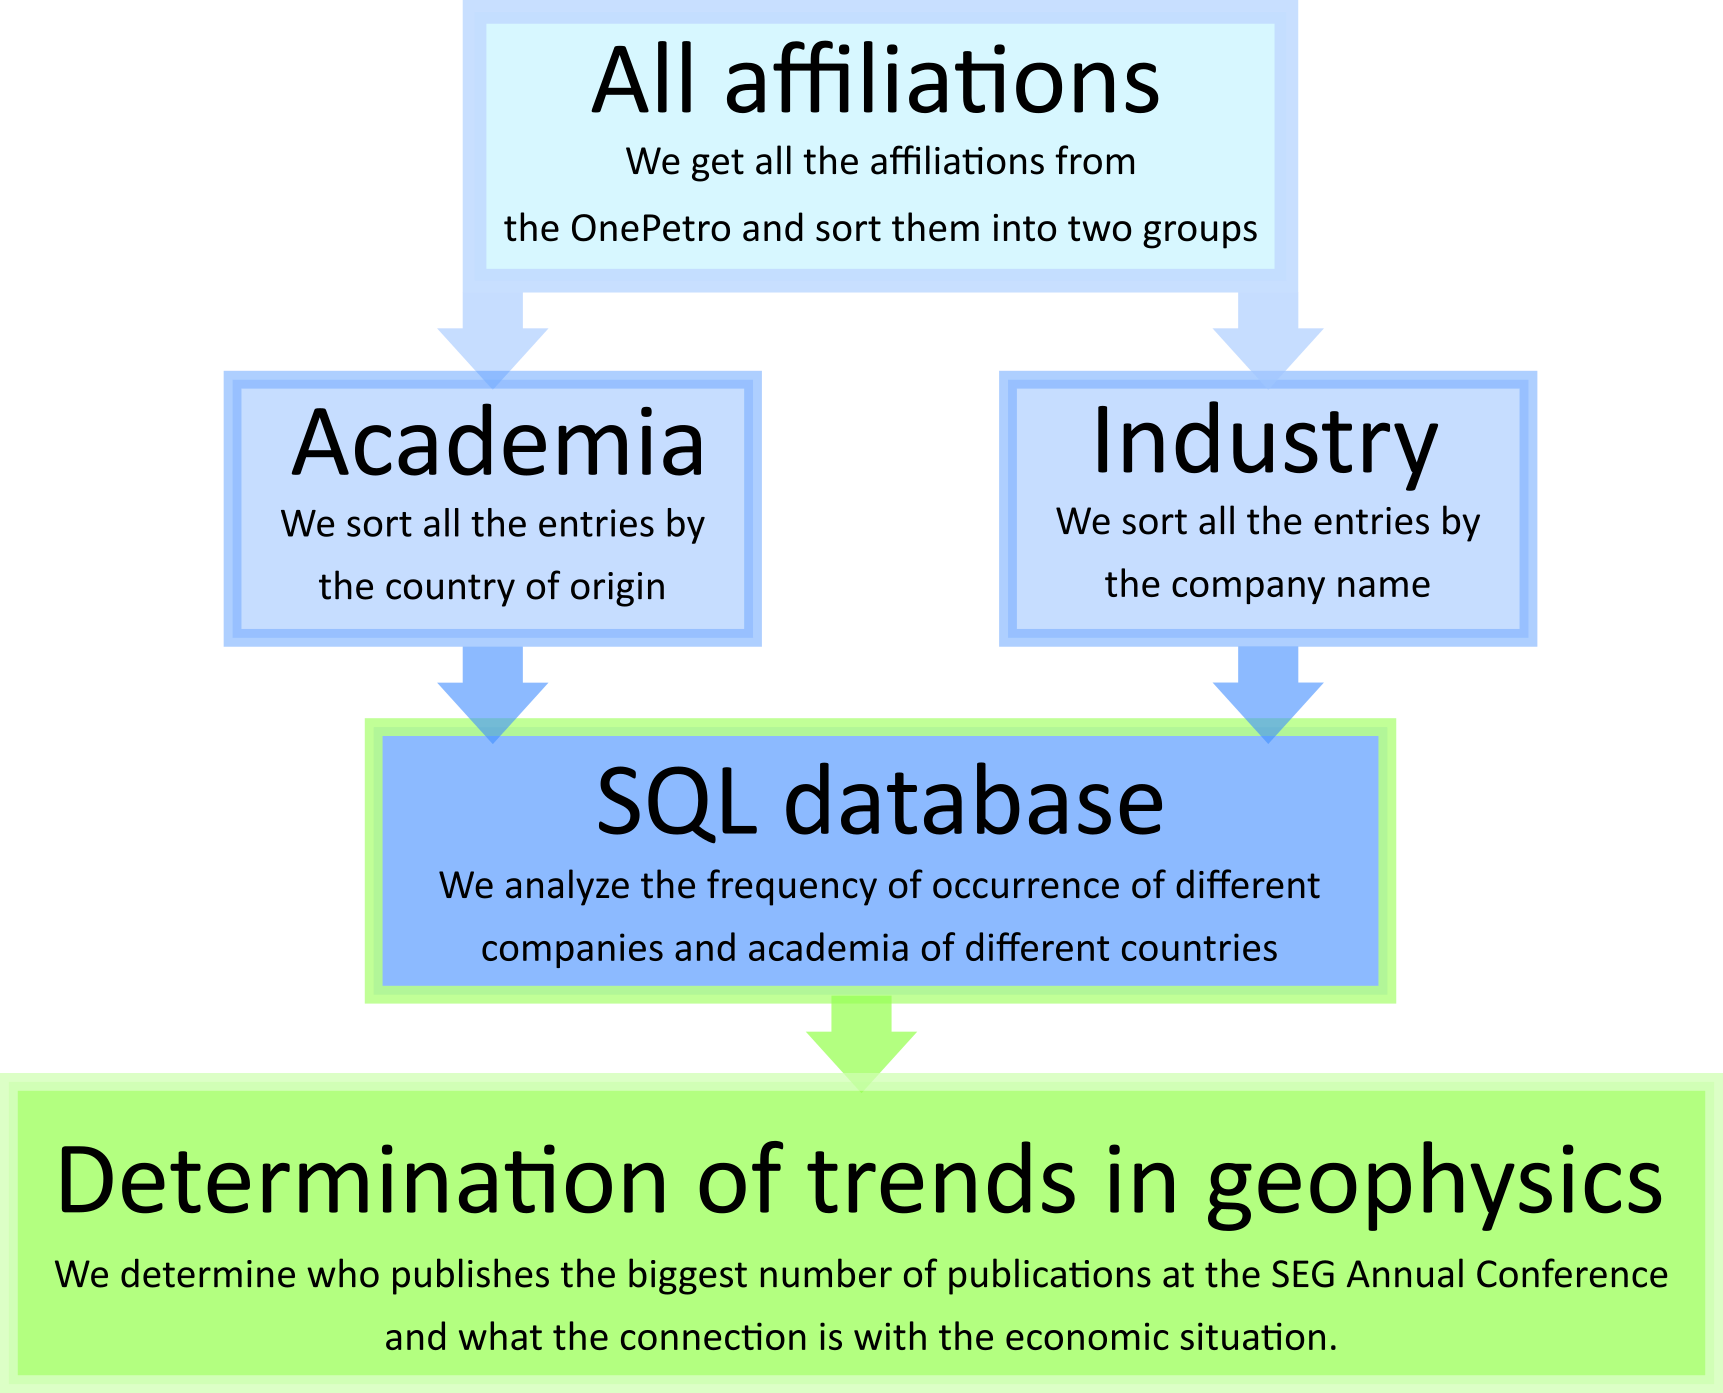
\includegraphics[scale=1]{scheme_meta.png}
\caption{Data processing workflow.}
\label{scheme_workflow}
\end{figure}


In total, we analyzed 24,500 papers for the 38 years period. The number of non-unique authors for the entire time span chosen in this paper exceeds 75 thousand. Fig. \ref{scheme_workflow} shows the data processing workflow. We received metadata for all 38 conferences and sorted them into academia and industry. After that, we sorted all affiliations from the industry into various companies and academic affiliations by various countries. Not all affiliations were complete; sometimes they looked like ``University of'', ``Geological Institute'', ``Unive'', ``Faculty of Geology and Mining'' \textit{etc.} This did not allow us to determine the country of such an institution, while it was clear that this was an academic institution. In this case, we define such an affiliation as an ``unknown academic institution'' and included it in a special list. 

After initial filtration, we count the number of affiliations per year from each particular company or academia of a particular country and analyze the change during time. The average number of authors per paper is growing over the years. There are many articles written jointly by authors from different companies. We divided the total number of affiliations from all the industrial companies and the academia by the average number of co-authors for each year. If one author used multiple affiliations, we took into account only the first mentioned. It is easy to identify large company affiliations and typos in the spelling of their names; it is most difficult to analyze industrial companies that published less than 10 times. Since the authors of these publications often allowed different spelling of their company name, we distributed them into different groups. We take note of the number of typographical errors of the  Schlumberger company name. It truly ranks first among all other companies: ``Schiumberger'', ``Schulmberger'', ``Shlumberger'', ``Schlumbeger'', ``Schlumbrrger'' \textit{etc.} The errors are partly due to carelessness and  incorrect machine recognition, but it is worth paying tribute to the Schlumberger company, which published the highest number of articles over the observed period.

 
%%%%%%%%%%%%%%%%%%%%%%%%%%%%%%%%%%%%%%%%%%
\section{Results}
%\subsection{Academia and Industry}

Fig. \ref{acad_world} reveals the average number of papers for academia by country. Each country is represented by a unique color; the size of the circles is the average number of publications. The inset in the lower-left corner shows a Europe zoom-in. The most considerable contribution is from the universities in the United States of America (the USA, see the five above) followed by universities in China (China University of Petroleum, Jilin University, and Tongji University), and Canada (University of British Columbia). The rest is shared among the Netherlands, France, Germany, and Russia.

China holds the leading position in Asia, followed by smaller but notable contributions from South Korea, Japan, and India. In South America, Brazil academia published the highest number of abstracts. In the Middle East, the most represented country at the SEG Annual Meetings over the past ten years is the Kingdom of Saudi Arabia. In 2009 the average number of publications was about one, and in 2019, it is more than 23, which is indeed impressive. None of the academia of the other countries have shown such rapid relative growth in recent years. The total number of publications from the top-50 countries is presented in the appendix, and the full list can be accessed here \citep{Eltsov2020}.

The circle on Antarctica represents incomplete affiliations or affiliations with typos that were not correctly recognized; therefore, it was impossible to determine the location. It provides an estimate of the total error of the analysis.

\begin{figure}[ht!]
\centering
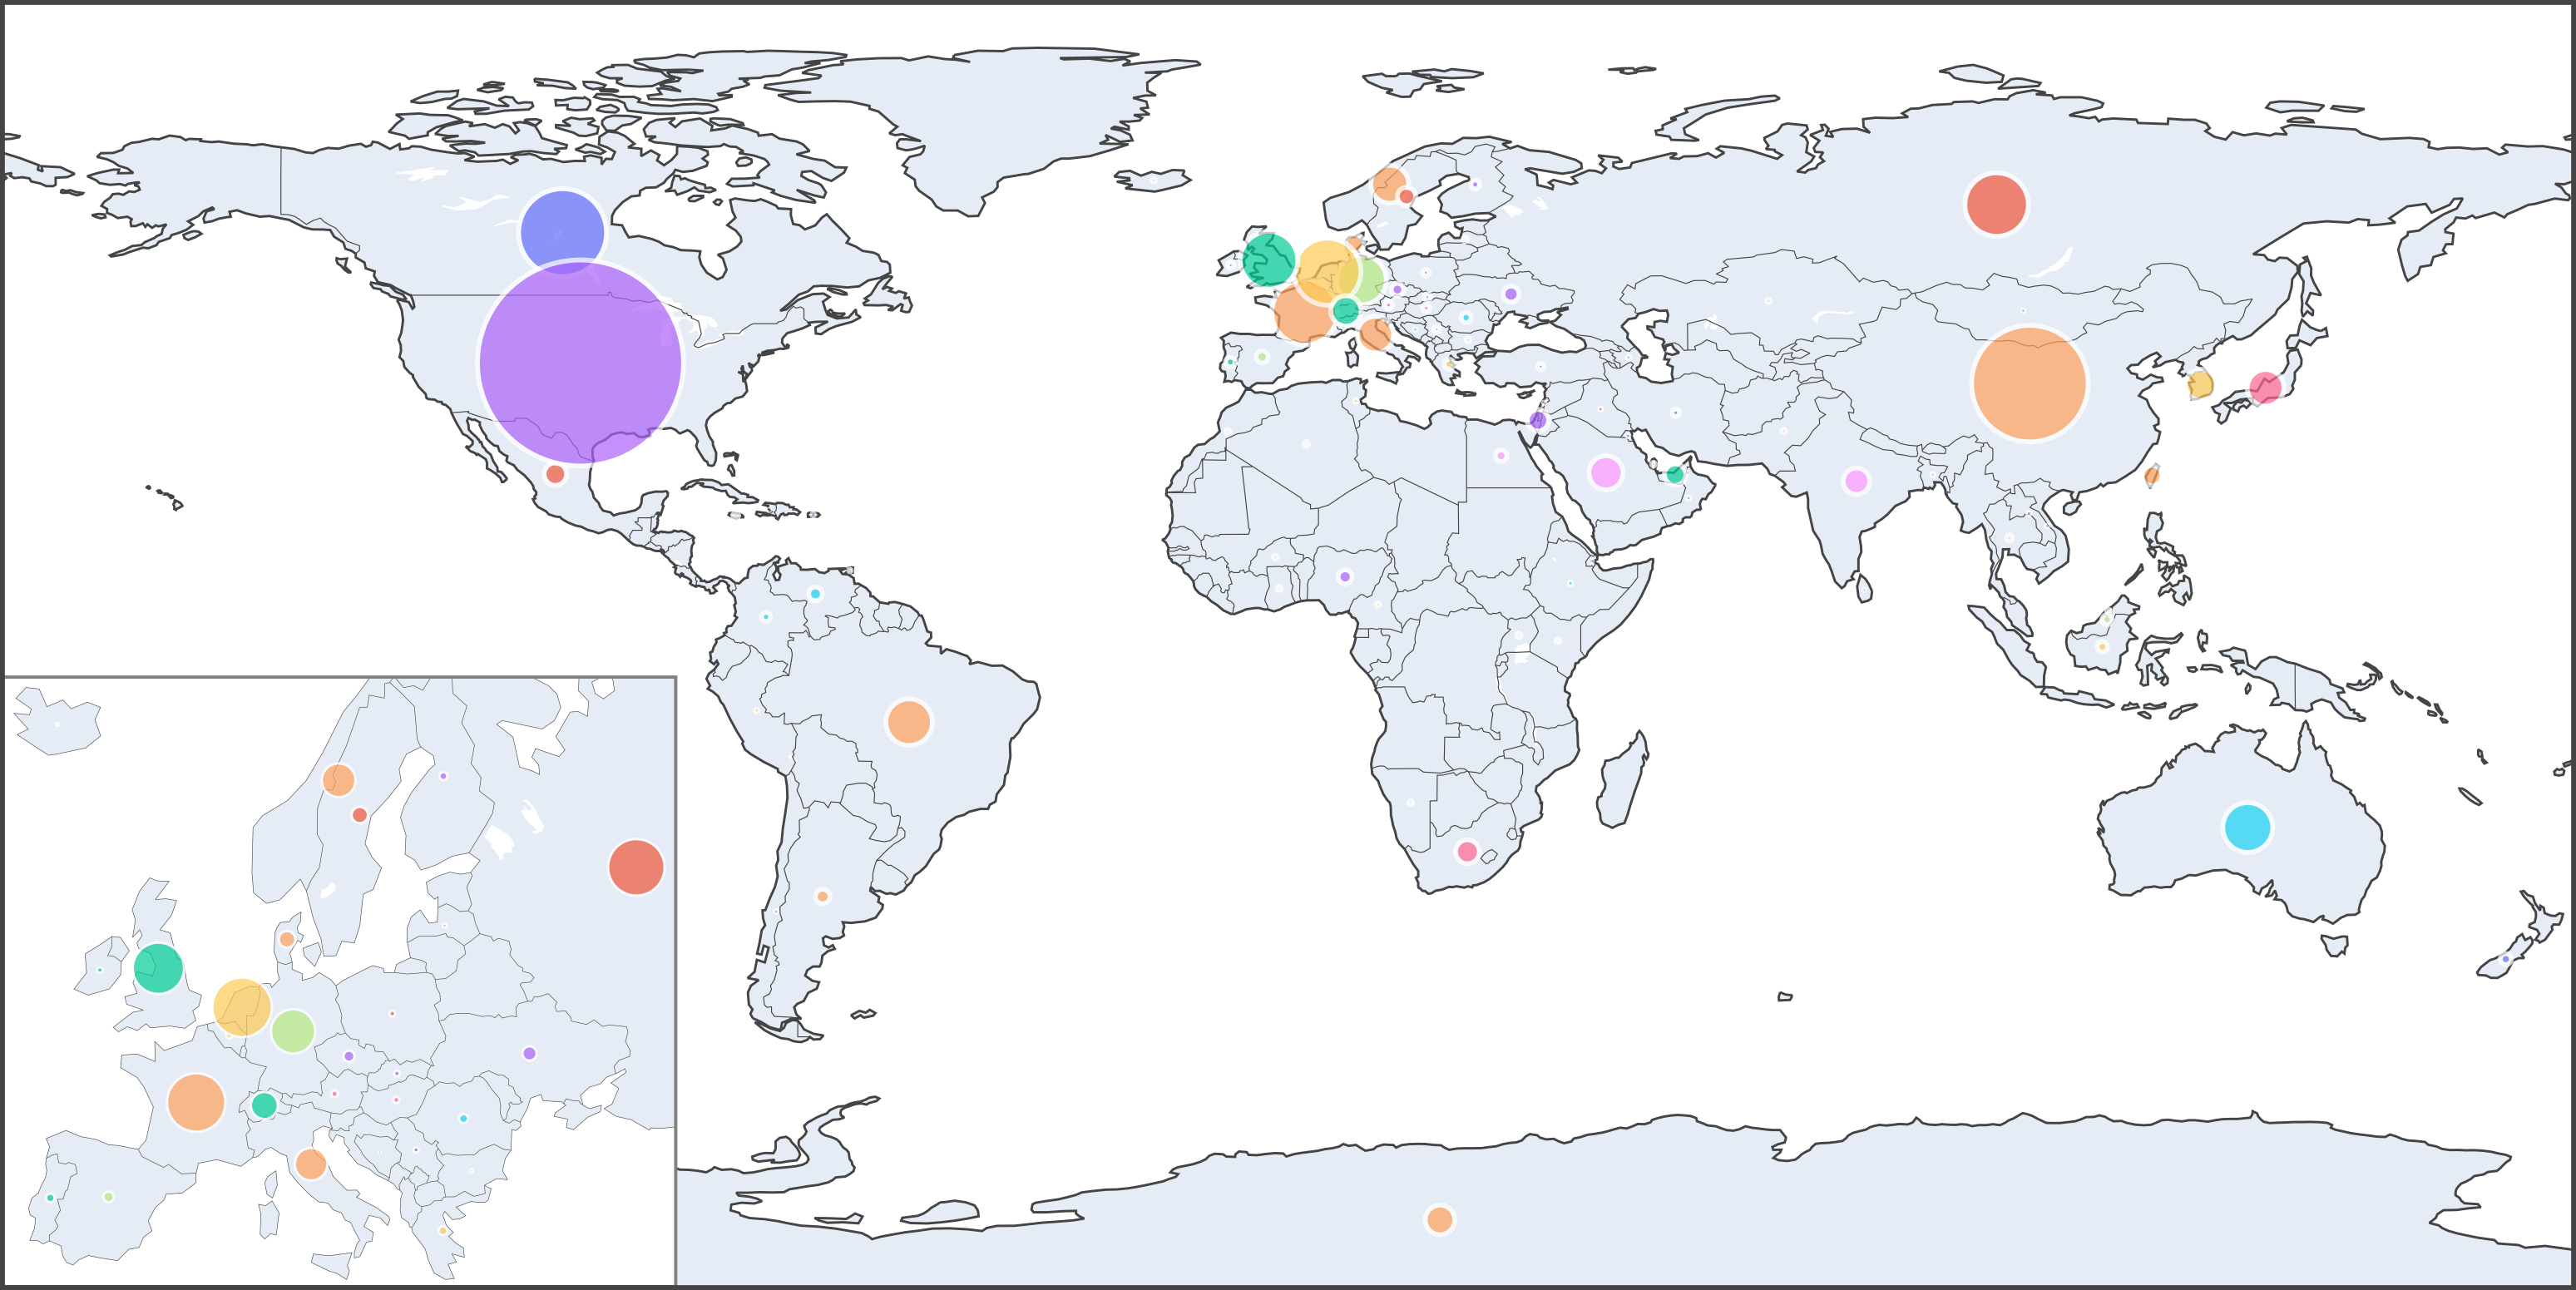
\includegraphics[width=\textwidth]{plottly_world3.png}
\caption{The total number of academic publications by country. Europe is in the zoomed inset on the lower left. The circle on Antarctica represents erroneous affiliations and serves as an error indicator.}
\label{acad_world}
\end{figure}

\begin{figure}[ht!]
\centering
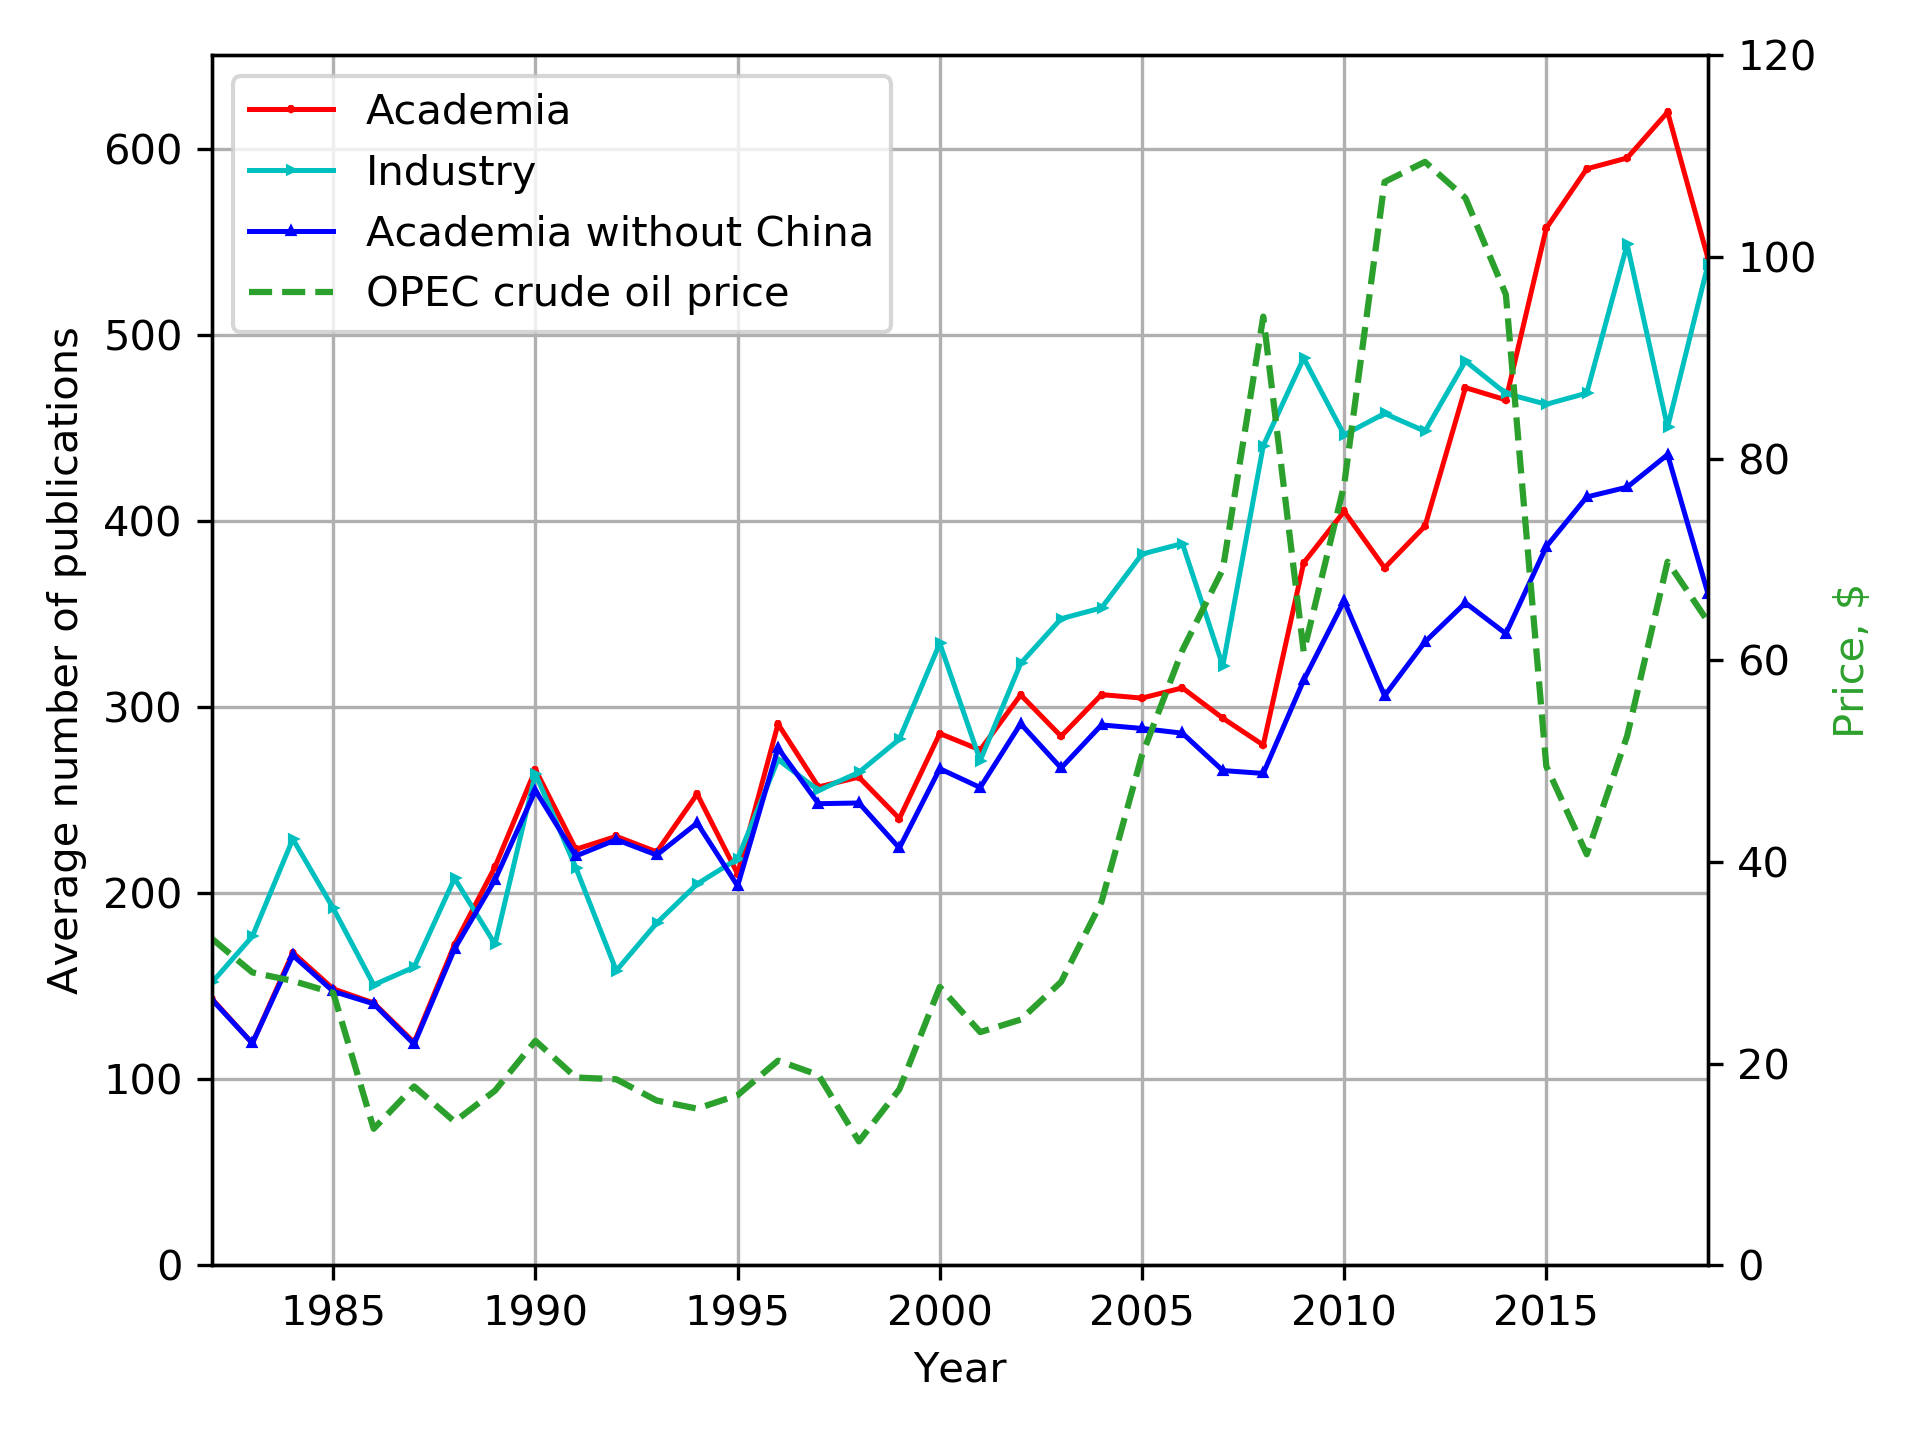
\includegraphics[scale=0.7]{acad_indus_plot.png}
\caption{The annual breakdown of net industry and academia publications.}
\label{acad_vs_ind}
\end{figure}

Fig. \ref{acad_vs_ind} compares the annual number of publications from industry and academia. Both contributors show a steady growth over the years, which is associated with an increase in fossil fuel consumption, oil price, and constant-growth-economic paradigm. However, on the finer scale, there is a weak correlation with the oil price change. For example, the number of academic publications was hardly affected by the two recent crises in 2008 and 2014. On average, the number of industrial publications is only partially influenced by the oil price dynamics resulting in a slower growth rate in the last few years. It appears that, on average, industry became more efficient in research expenditure optimization, which enabled them to maintain a high number of publications and even a slow but consistent growth during the shrinking market.

Curiously, the number of publications from academia in 2019 fell significantly. Fig. \ref{acad_vs_ind} indicates a decrease in the number of publications from the USA academia in 2019 compared to 2018. Perhaps this was due to a reduction in state funding of higher educational institutions \citep{Brownstein2018}; see blue curve drop in 2018-2019 Fig. \ref{acad_countries4}.


Fig. \ref{co_auth} shows that the number of co-authors per paper has increased, and we observe a correlation with the world trend exemplified by a related field of the Earth and Planetary sciences. The increase in the number of authors per paper is a worldwide trend \citep{Mallapaty2018}; scientific research is becoming more interdisciplinary and thus more collaborative. The SEG average co-author number almost flattens out at 3.6 co-authors per paper, but in 2019 the number of authors per paper increased, reaching 3.9. With that, we see an increase in the number of organizations involved in the SEG Annual Conference.

\begin{figure}[ht!]
\centering
\includegraphics[scale=0.7]{Co_auth.png}
\caption{Number of co-authors growth rate for the SEG Annual Conference and for the Earth and Planetary science \citep{Mallapaty2018}.}
\label{co_auth}
\end{figure}

More than 2400 industry companies and academic institutions from eighty-six countries have presented their research at the SEG Annual Conference so far. The five companies with the most significant number of publications in the SEG Annual Conference are 1) Schlumberger, 2) WesternGeco, 3) CGG (Compagnie Générale de Géophysique), 4) BGP Inc. (BGP Inc., China National Petroleum Corporation), and 5) BP plc (formerly The British Petroleum Company plc and BP Amoco plc). These five companies accounted for about 30\% of all affiliations in the past ten years. Schlumberger constitutes about 8\% of all affiliations, with WesternGeco adding about 5\% in the past ten years. Fig. \ref{companies_hist} breaks down the number of companies with the corresponding number of publications. There are only two companies that on average have published more than 500 publications (Schlumberger and CGG), and there are more than 2100 companies that published five papers and less. The number of companies that have published less than five papers over the years is gradually growing \citep{Eltsov2020}. 


\begin{figure}[ht!]
\centering
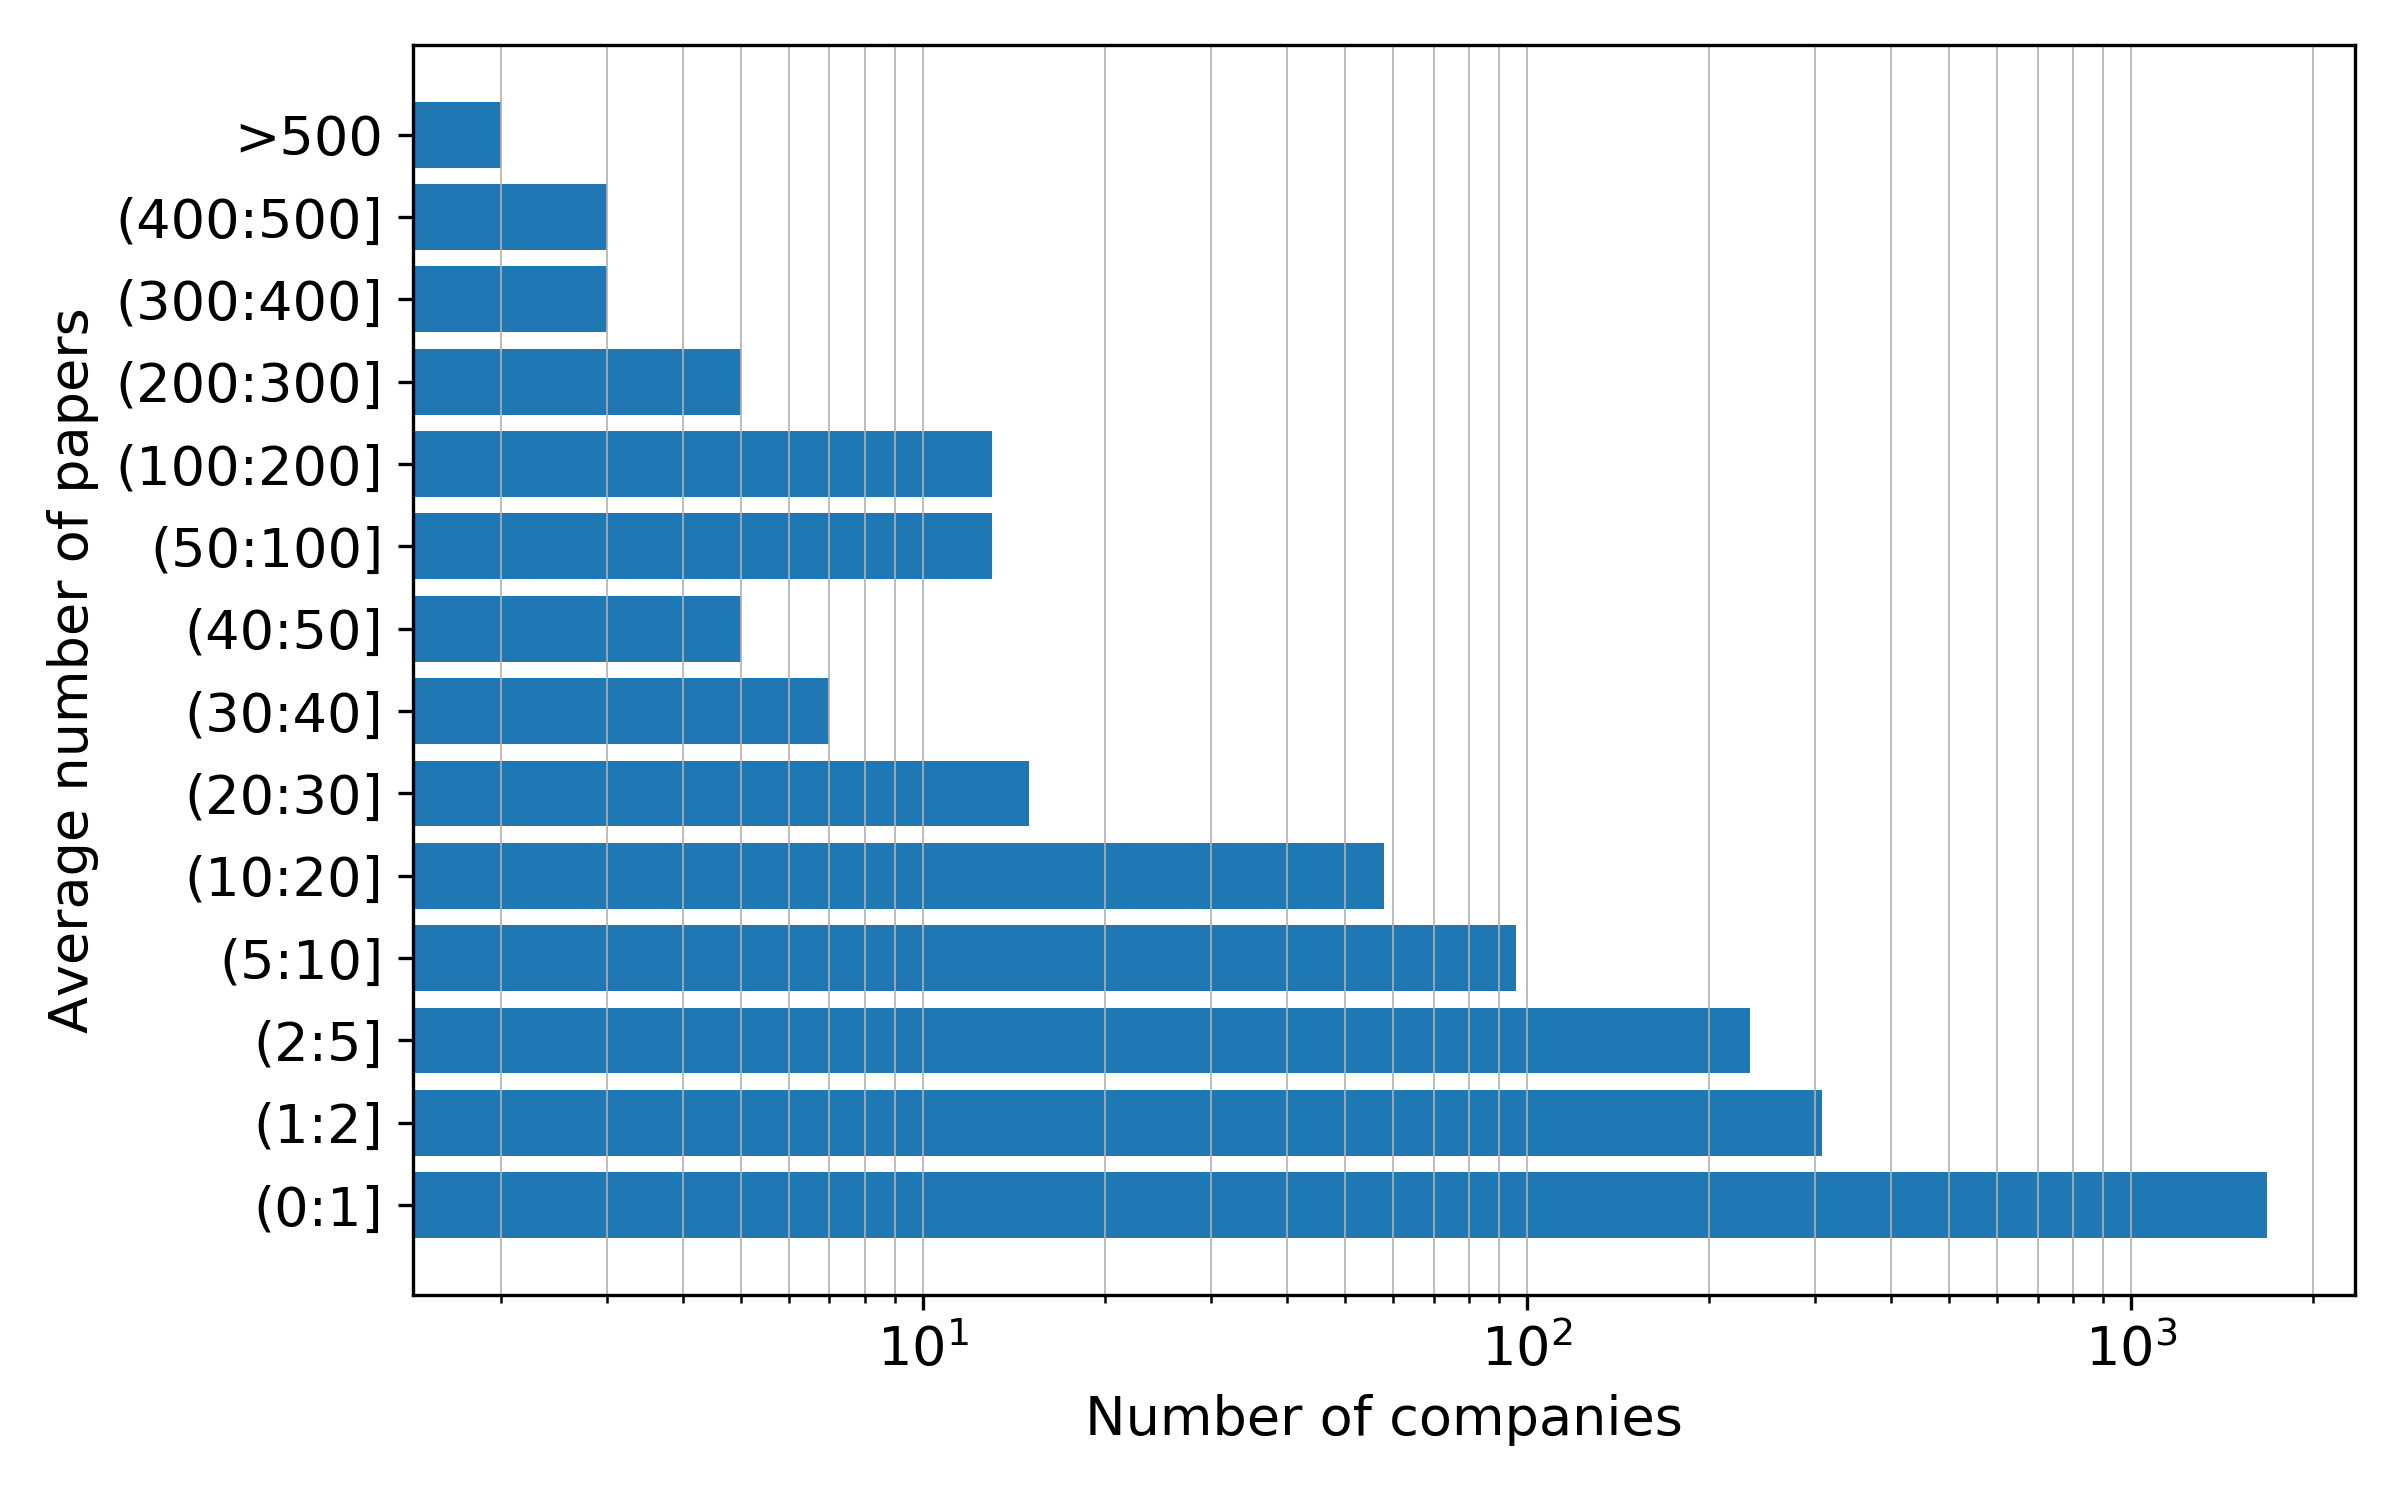
\includegraphics[scale=0.7]{companies_hist.png}
\caption{Average number of paper vs. number of companies that publish the papers.}
\label{companies_hist}
\end{figure} 
 
The five most highly represented universities in SEG Annual Conferences over the 38 years are 1) Colorado School of Mines, 2) University of Houston, 3) China University of Petroleum, 4) Stanford University, and 5) Delft University of Technology. 


Fig. \ref{acad_countries4} shows a breakdown of academic publications by country. The USA academia is ahead of everyone in the number of papers published annually, as well as the total articles published. The Netherlands and Canada, have regular contributions, and their publication activity is constant over time. Other countries, like France and Germany, seem to follow the crude oil price trend. In contrast, China maintains a steady growth rate. In 2006 the Chinese government initiated a powerful program of research development, ``Medium and Long-term Plan for the Development of Science and Technology (2006–2020)'' with a target of 2.5\% GERD/GDP ratio by 2020 \citep{UNESCO2015}. The strong support of the government for geoscience, allowed the Chinese academia to exhibit the fastest growth between 2008 and 2015. In 2013, we observed a 15\% increase in R\&D spending by China compared to 2012 \citep{Ni2015}. The number of publications by the Chinese academia is now almost equal to those of the USA.


\begin{figure}[ht!]

\begin{overpic}[abs,unit=1mm,width=\textwidth]{4_first_countries.png}
\put(139,70){\citep{Brownstein2018}}
\put(151.5,40.8){\citep{Ni2015}}
\put(150.9,15.3){\citep{UNESCO2015}}
\end{overpic}

\caption{Average number of publications by academia of the TOP-four countries.}
\label{acad_countries4}
\end{figure}


\begin{figure}[ht!]
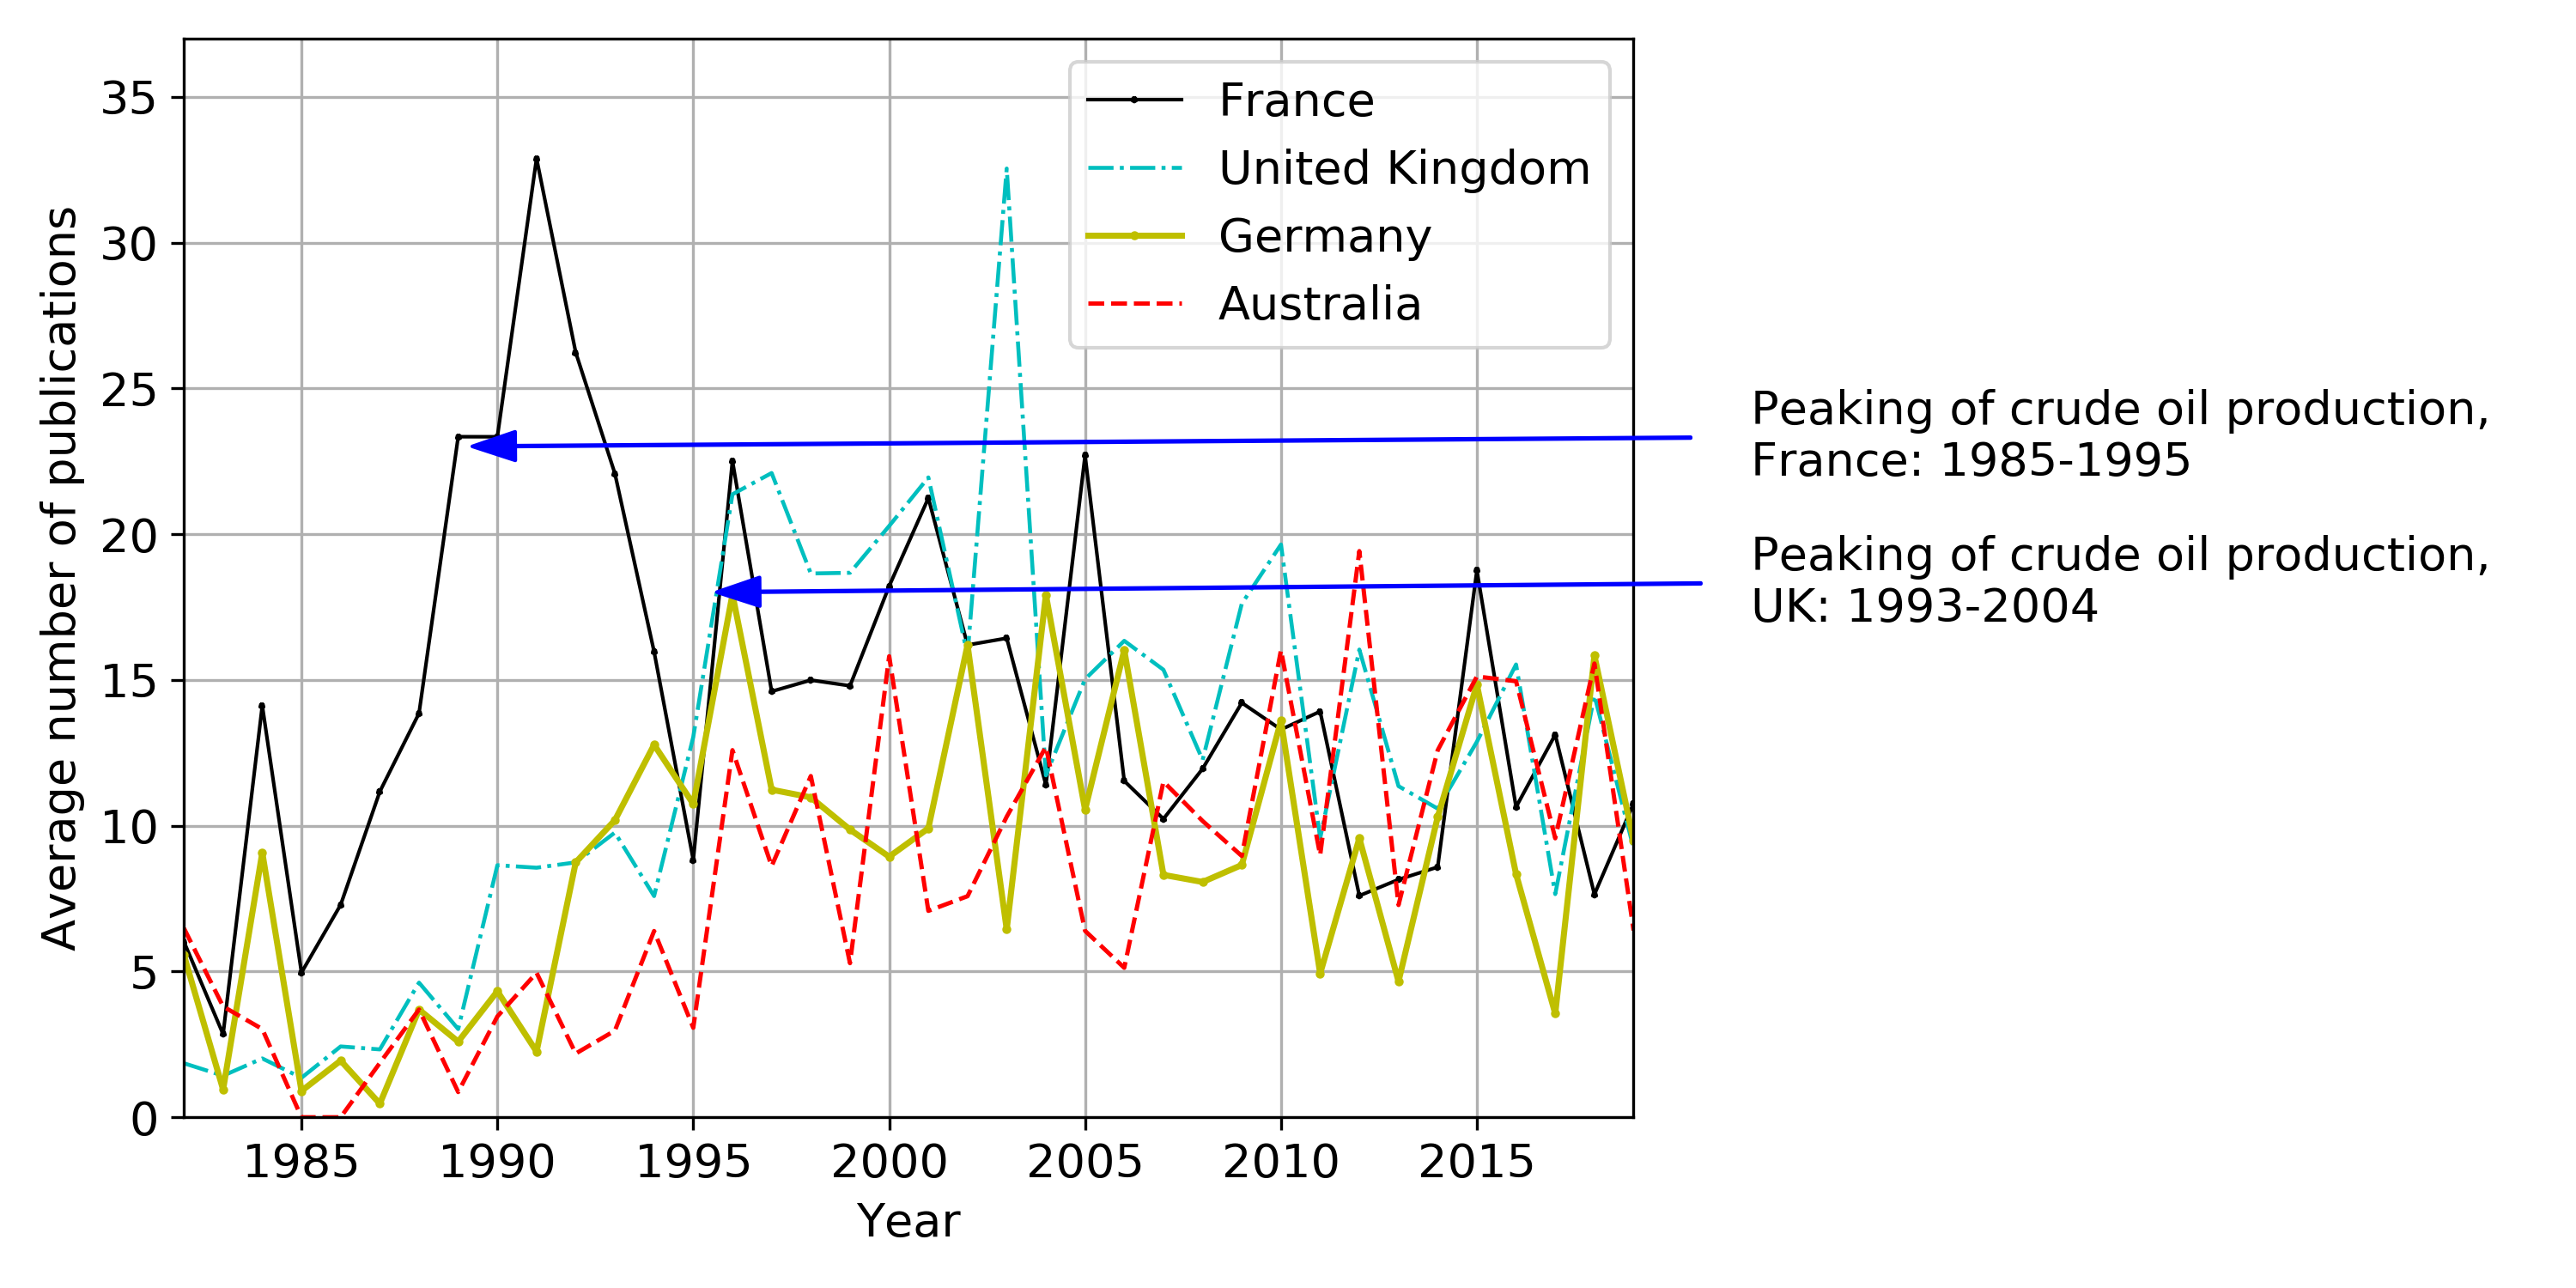
\includegraphics[width=\textwidth]{4_second_countries.png}
\caption{Average number of publications by France, UK, Germany, and Australia. Crude oil production data is presented online \citep{CEIC2020}.}
\label{acad_countries8}
\end{figure}


Next, we perform a similar analysis for industry publications. Fig. \ref{serv_comp} shows the average number of papers by oilfield service companies. The most frequent guests at the SEG Annual Conferences are Schlumberger, WesternGeco, CGG, and BGP. Although WesternGeco is a part of Schlumberger, we show them separately according to the affiliation. Schlumberger dominates industrial geophysics research, followed by CGG and BGP. In general, the number of publications by the major oilfield service companies grew steadily. Although oilfield service providers are dependent on oil prices, we surprisingly observe that after the 2014 crisis, the number of Schlumberger publications peaked for several consecutive years \citep{Schlumberger2014}, followed by a decline in 2018. It should be noted that in 2014 Schlumberger reported an outstanding revenue of \$48.6 billion. The dynamics of Schlumberger's papers reflect the dynamics of oil prices with a few years offset. The number of CGG publications follows crude oil prices too, but since 2014, the number of publications from CGG has only declined. CGG Annual report states extremely difficult market environment \citep{CGG2015}, and cost reduction measures: reduction in the number of employees from 11060 to 7353, 55\% general and administrative cost-cutting, 64\% cost of marine monthly structure cost-cutting\footnote{A comparison of 2013 and 2015 indicators}. In January 2020, CGG reported its exit from marine acquisition, sale of ships and measuring equipment to Shearwater company \citep{CGG2020}. This news suggests that we will see fewer publications from CGG in the coming years. 

The change in the number of BGP publications shows a similar trend with the crude oil prices with one or two years of delay. In 2019 BGP became a leader by the number of publications among oil service providers.

\begin{figure}[ht!]


\begin{overpic}[abs,unit=1mm,width=\textwidth]{Oil_service.png}
\put(146,68.5){\citep{Schlumberger2014}}
\put(142,30){\citep{CGG2015}}
\end{overpic}

\caption{The average number of publications by oil-service companies and OPEC crude oil prices.}
\label{serv_comp}
\end{figure}

\begin{figure}[ht!]

\begin{overpic}[abs,unit=1mm,width=\textwidth]{oil_companies.png}
\put(141.5,67){\citep{Aramco2018}}
\put(140.3,50.5){\citep{ExxonMobil2005}}
\put(133.5,14){\citep{ExxonMobil2014}}
\end{overpic}

\caption{The average number of publications by oil production companies.}
\label{oil_comps}
\end{figure}


Many oil and gas companies that no longer exist made significant contributions to the SEG Annual Conference in the 1980s and early 1990s. They are Arco Oil and Gas Co., Mobil E\&P, OYO Corporation, Statoil, and others. These companies either merged with others, changed their names, or were acquired.

Fig. \ref{oil_comps} displays five oil production companies with the most significant number of publications. The picture is conceptually different from oil service companies. For example, the number of publications by BP and ExxonMobil peaked in 2005 and nowadays, it is declining. 2005 was an outstanding year for ExxonMobil, with a net income of 36 billion and a 31\% increase in the number of employees \citep{ExxonMobil2005}. We observe steady growth in many economic indicators of the company since the beginning of 2000. At the same time, a decrease in the number of publications indicates a difficult period for the company. For instance, in 2014, we found only one paper from ExxonMobil, which has not happened over the past 15 years. The 2014 ExxonMobil Summary Annual Report \citep{ExxonMobil2014} shows that compared to 2013, market valuation at the end of the year decreased by 12\%, and we observe the decline in the stock market price of ExxonMobil in 2015. The decrease in profits immediately affects research financing. Saudi Aramco demonstrates steady growth; it had the biggest number of publications of all production companies in 2017 and 2018. Interestingly enough, the leadership was taken by PetroChina in 2019, followed by Shell and Saudi Aramco.


%%%%%%%%%%%%%%%%%%%%%%%%%%%%%%%%%%%%%%%%%%%
%\section{Discussion}
%
%The amount of hidden information is astounding. Such a study is unique because we have at our disposal a history of the development of geophysics. 


%%%%%%%%%%%%%%%%%%%%%%%%%%%%%%%%%%%%%%%%%%
\section{Conclusions}

We analyzed metadata of 24,500 papers prepared by more than 75,000 authors for     the 38 years. Academic institutions from 86 countries and more than 2400 industrial companies contributed to the SEG Annual Conference from 1982 to 2019. The USA academia has the most significant impact in the proceedings of the SEG Annual Conference during the whole observation period. We observe that the number of papers from the Chinese academia is growing, and it is almost equal to those of the USA. The activity of the companies at the SEG Annual Conference shows their economic condition, annual reports by CGG and ExxonMobil and other companies confirm this statement. Depending on the financial situation on the market, and the price of oil, the contribution of the academia and industry by publications changes in time. Over time, the number of companies that publish a small number of papers is growing. In 2018 we observed more abstracts from the academia, but in 2019 the number of publications from academia and industry was very close. In 2019 the most significant number of publications in the industry was made by BGP and PetroChina. The average number of authors per paper continues to grow over time in agreement with the global trend of Earth and Planetary science, but at a slower rate. Analysis of publication activity is a unique approach to processing large amounts of data, and the authors propose using this approach in other areas of the national economy.


%%%%%%%%%%%%%%%%%%%%%%%%%%%%%%%%%%%%%%%%%%
\vspace{6pt} 

%%%%%%%%%%%%%%%%%%%%%%%%%%%%%%%%%%%%%%%%%%
\authorcontributions{Data mining and processing, software development, original draft preparation - Timofey Eltsov; software development and analysis, review and editing of the draft - Maxim Yutkin; supervision, project administration, historical analysis, review, and editing of the paper - Tadeusz W. Patzek.}

%%%%%%%%%%%%%%%%%%%%%%%%%%%%%%%%%%%%%%%%%%
\funding{Dr. Eltsov was supported by the KAUST Magnetic Sensor project, REP-2708.}

%%%%%%%%%%%%%%%%%%%%%%%%%%%%%%%%%%%%%%%%%%
\acknowledgments{The authors are grateful to their colleagues, and especially to Dr. Thomas Finkbeiner, for valuable and vital research recommendations. The authors are grateful to Ilya Kolganov for the useful advice on the design of the graphs. We also would like to acknowledge Dr. Charles Russell Severance for an informative Python course.}

%%%%%%%%%%%%%%%%%%%%%%%%%%%%%%%%%%%%%%%%%%
\conflictsofinterest{The authors declare no conflict of interest.} 

%%%%%%%%%%%%%%%%%%%%%%%%%%%%%%%%%%%%%%%%%%
%% optional
\abbreviations{The following abbreviations are used in this manuscript:\\

\noindent 
\begin{tabular}{@{}ll}
ASCII & American standard code for information interchange\\
BP & BP plc., formerly The British Petroleum Company and BP Amoco\\
CGG & Compagnie Générale de Géophysique \\
CMP & Common Mid Point\\
EAGE & European Association of Geoscientists and Engineers\\
GB & Giga Byte\\
GDP & Gross Domestic Product\\
GERD & Gross domestic Expenditure on Research and Development\\
HTML & HyperText Markup Language\\
ICT & Information and Communication Technology \\
KTH & KTH Royal Institute of Technology in Stockholm\\
NLTK & Natural Language Toolkit\\
NMO & Normal Moveout\\
PDF & Portable Document Format \\
PIL & Python Imaging Library\\
R\&D & Research and Development\\
SEG & Society of Exploration Geophysicists\\
SPE & Society of Petroleum Engineers\\
SPWLA & Society of Petrophysicists and Well Log Analysts \\
Wt & Watt\\
USA & The United States of America\\
ZB & Zetta Byte
\end{tabular}}
%%%%%%%%%%%%%%%%%%%%%%%%%%%%%%%%%%%%%%%%%%
%% optional
\appendixtitles{yes} %Leave argument "no" if all appendix headings stay EMPTY (then no dot is printed after "Appendix A"). If the appendix sections contain a heading then change the argument to "yes".
\appendix
\section{The total number of publication by country}
\begin{tabular}{@{}p{0.5cm}<{}@{}p{9cm}<{\dotfill}@{}p{\dimexpr\linewidth-4cm}@{}}
\textbf{\#} & \textbf{Country name} & \textbf{The total number of publications} \\
1 & United States of America & 5154.07\\
2 & China & 1649.95\\
3 & Canada & 952.47\\
4 & Netherlands & 608.58\\
5 & France & 546.53\\
6 & United Kingdom of Great Britain and Northern Ireland & 462.14\\
7 & Germany & 330.39\\
8 & Australia & 302.54\\
9 & Brazil & 264.0\\
10 & Japan & 205.62\\
11 & Russian Federation & 178.75\\
12 & Norway & 176.36\\
13 & Italy & 164.11\\
14 & Saudi Arabia & 145.46\\
15 & Korea, Republic of & 138.62\\
16 & Switzerland & 113.01\\
17 & India & 99.08\\
18 & Mexico & 62.15\\
19 & Denmark & 57.58\\
20 & Israel & 55.69\\
21 & Taiwan & 49.44\\
22 & Sweden & 41.45\\
23 & Venezuela (Bolivarian Republic of) & 28.01\\
24 & Argentina & 25.78\\
25 & South Africa & 24.53\\
26 & Nigeria & 23.96\\
27 & United Arab Emirates & 19.75\\
28 & Czechia & 19.34\\
29 & Spain & 17.86\\
30 & Egypt & 16.52\\
31 & Singapore & 14.98\\
32 & New Zealand & 14.77\\
33 & Romania & 13.7\\
34 & Indonesia & 13.42\\
35 & Malaysia & 12.66\\
36 & Greece & 12.06\\
37 & Portugal & 11.74\\
38 & Ukraine & 11.08\\
39 & Colombia & 10.25\\
40 & Finland & 9.8\\
41 & Austria & 6.92\\
42 & Iran & 6.78\\
43 & Belgium & 5.43\\
44 & Slovakia & 5.35\\
45 & Ireland & 5.26\\
46 & Poland & 5.22\\
47 & Turkey & 5.2\\
48 & Serbia & 4.5\\
49 & Thailand & 4.34\\
50 & Jamaica & 4.32\\
\end{tabular}

%\unskip
%\subsection{}
%The appendix is an optional section that can contain details and data supplemental to the main text. For example, explanations of experimental details that would disrupt the flow of the main text, but nonetheless remain crucial to understanding and reproducing the research shown; figures of replicates for experiments of which representative data is shown in the main text can be added here if brief, or as Supplementary data. Mathematical proofs of results not central to the paper can be added as an appendix.
%%
%\section{}
%All appendix sections must be cited in the main text. In the appendixes, Figures, Tables, etc. should be labeled starting with `A', e.g., Figure A1, Figure A2, etc. 

%%%%%%%%%%%%%%%%%%%%%%%%%%%%%%%%%%%%%%%%%%
\reftitle{References}

% Please provide either the correct journal abbreviation (e.g. according to the "List of Title Word Abbreviations" http://www.issn.org/services/online-services/access-to-the-ltwa/) or the full name of the journal.
% Citations and References in Supplementary files are permitted provided that they also appear in the reference list here. 

%=====================================
% References, variant A: external bibliography
%=====================================
%\externalbibliography{yes}
%\bibliography{your_external_BibTeX_file}
%\bibliography{timaref}
%=====================================
% References, variant B: internal bibliography
%=====================================
\begin{thebibliography}{999}
\providecommand{\natexlab}[1]{#1}

\bibitem[Reinsel \em{et~al.}(2018)Reinsel, Gantz, and Rydning]{Reinsel2018}
Reinsel D.; Gantz J.; Rydning J.
\newblock {The Digitization of the World From Edge to Core}. \newblock {Available online: https://www.seagate.com/files/www-content/our-story/trends/files/idc-seagate-dataage-whitepaper.pdf/ (Accessed on 4 March 2020)}


\bibitem[Costenaro \em{et~al.}(2012)Costenaro, and Duer]{Costenaro2012}
Costenaro D.; Duer A.
\newblock {The Megawatts behind Your Megabytes: Going from Data-Center to Desktop}. \newblock {Available online: https://www.aceee.org/files/proceedings/2012/data/papers/0193-000409.pdf (Accessed on 4 March 2020)}

\bibitem[Van Heddeghem \em{et~al.}(2014)Van Heddeghem, Lambert, Lannoo, Colle, Pickavet, and Demeester]{Heddeghem2014}
Heddeghem, V. W.; Lambert, S.; Lannoo, B.; Colle, D.; Pickavet, M.; Demeester, P.
\newblock {Trends in worldwide ICT electricity consumption from 2007 to 2012}.
\newblock {\em Computer Communications} {\bf 2014}, {\em 50}, {9}, ~64--76.
\newblock
 doi:{\changeurlcolor{black}\href{https://doi.org/10.1016/j.comcom.2014.02.008}{\detokenize{10.1016/j.comcom.2014.02.008}}}.


\bibitem[Dulac \em{et~al.}(2012)Dulac, Abergel, and Delmastro]{Dulac2019}
Dulac J.; Abergel T.; Delmastro C.
\newblock {Data centres and data transmission networks}. \newblock {Available online: https://www.iea.org/reports/tracking-buildings/data-centres-and-data-transmission-networks (Accessed on 4 March 2020)}

\bibitem[(2019)]{KTH2019}
\newblock {Internet drar 10\% av världens elanvändning - och andelen stiger}. \newblock {Available online: https://cornucopia.cornubot.se/2019/02/internet-drar-10-av-varldens.html?m=1 (Accessed on 4 March 2020)}

\bibitem[BP (2019 )]{BP2019}
BP.
\newblock {\emph{BP Statistical Review of World Energy, 68th edition}};
\newblock Report; {Pureprint Group Limited, UK}, 2019 .


\bibitem[SEG, (2019)]{SEG}
\newblock {SEG Technical Program Expanded Abstracts. Available online: https://library.seg.org/series/segeab (Accessed on 2 December 2019)}.

\bibitem[OnePetro, (2019)]{SPE2019}
\newblock {OnePetro online library. Available online: https://www.onepetro.org (Accessed on 2 December 2019)}.


\bibitem[Eltsov (2020)]{Eltsov2020}
Eltsov, T.
\newblock {Data for SEG Annual Conferences analysis, 1982 - 2019. Available online: https://github.com/ANPERC-source/SEG\_Annual (Accessed on 2 February 2020)}.


\bibitem[American Higher Education Hits a Dangerous Milestone, (2018)]{Brownstein2018}
\newblock {American Higher Education Hits a Dangerous Milestone}. \newblock {Available online: https://www.theatlantic.com/\\politics/archive/2018/05/american-higher-education-hits-a-dangerous-milestone/559457/ (Accessed on 2 December 2019)}
%author = {Brownstein, Ronald},
%shorturl.at/PRWYZ (Accessed on 2 December 2019)}.

\bibitem[Mallapaty (2018)]{Mallapaty2018}
\newblock {Paper authorship goes hyper. Available online: https://www.natureindex.com/news-blog/paper-authorship-\\goes-hyper (Accessed on 17 October 2019)}.


\bibitem[UNESCO (2015)]{UNESCO2015}
UNESCO.
\newblock {\emph{UNESCO SCIENCE REPORT, Towards 2030}};
\newblock Report; {United Nations Educational, Paris, France}, 2015.

\bibitem[Ni (2015)]{Ni2015}
Ni, X.
\newblock {China's research \& development spend}.
\newblock {\em Nature} {\bf 2015}, {\em 520}, {S8-S9}.
\newblock
 doi:{\changeurlcolor{black}\href{ https://doi.org/10.1038/520S8a}{\detokenize{10.1038/520S8a}}}.


\bibitem[CEIC (2020)]{CEIC2020}
\newblock {Global Economic Data, Indicators, Charts\& Forecasts, CEIC. Available online: https://www.ceicdata.com (Accessed on 10 February 2020)}.

\bibitem[Schlumberger(2014)]{Schlumberger2014}
Schlumberger.
\newblock {\emph{2014 Annual Report}};
\newblock Report; {Schlumberger: Paris, France} 2015.



\bibitem[CGG(2015)]{CGG2015}
Compagnie Générale de Géophysique
\newblock {\emph{ANNUAL REPORT 2015}};
\newblock Report; {CGG: Chicago, Ill., USA} 2015.

\bibitem[CGG (2020)]{CGG2020}
Compagnie Générale de Géophysique
\newblock {CGG completes its exit from marine acquisition. Available online: https://www.cgg.com/en/Investors/Press-Releases/2020/01/CGG-Completes-its-Exit-from-Marine-\\Acquisition (Accessed on 2 February 2020)}.

\bibitem[Saudi Aramco(2018)]{Aramco2018}
Saudi Aramco.
\newblock {Saudi Arabian Oil Company, Consolidated financial statements for the year ended december 31, 2018. Available online: https://www.saudiaramco.com/-/media/publications/corporate-reports/saudi-aramco-results-2017-2018\\-full-financials.pdf (Accessed on 11 February 2020)}.


\bibitem[ExxonMobil(2005)]{ExxonMobil2005}
ExxonMobil.
\newblock {\emph{Summary Annual Report 2005}};
\newblock Report; {ExxonMobil: Irving, TX, USA,} 2005.

\bibitem[ExxonMobil(2014)]{ExxonMobil2014}
ExxonMobil.
\newblock {\emph{Summary Annual Report 2014}};
\newblock Report; {ExxonMobil: Irving, TX, USA,} 2014.

\end{thebibliography}
%%%%%%%%%%%%%%%%%%%%%%%%%%%%%%%%%%%%%%%%%%
%% optional
%\sampleavailability{Samples of the compounds ...... are available from the authors.}

%% for journal Sci
%\reviewreports{\\
%Reviewer 1 comments and authors’ response\\
%Reviewer 2 comments and authors’ response\\
%Reviewer 3 comments and authors’ response
%}

%%%%%%%%%%%%%%%%%%%%%%%%%%%%%%%%%%%%%%%%%%
\end{document}


%%% Local Variables:
%%% mode: latex
%%% TeX-master: t
%%% End:
